%Description - Contains A description of how to make to script files battle each other, 

\section{ Description of The \textit{WAR}-Game }
\label{sec:describeWAR}
As mentioned earlier the \textit{WAR}-Game is a simulation where the players will program the behaviour of their armies with a script, and let the game being executed without further interaction. The winner of the simulation will be the one with the best script, as decided by the simulation engine. \\
	\subsection{The simulation}
	\begin{figure}
	\centering
	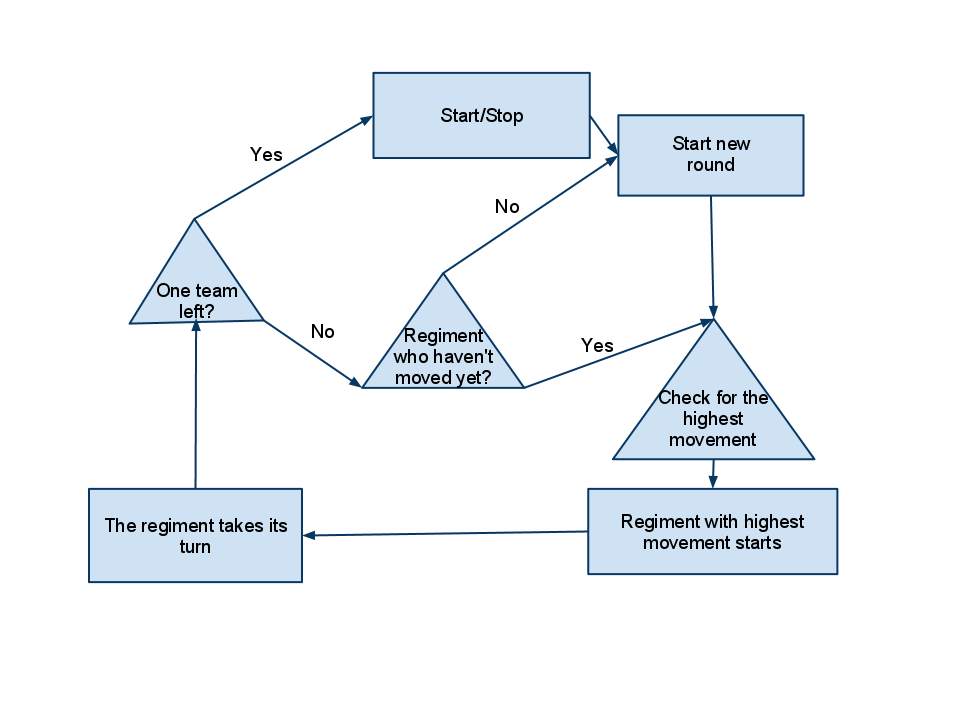
\includegraphics[scale=0.4]{rapport/2/figures/FlowChartSimulation}
	\caption{ Flowchart of the simulation } \label{fig:FlowChartSimulation}
	\end{figure}		
		To run a simulation in the \textit{WAR} simulation, a configuration file and at least two team files has to be fed to the simulation upon start up. 
		These files are written in the \textit{WAR} scripting language.
		\\
		The configuration file is used to establish basic rules for the war simulation, i.e. the size of the battlefield, the maximal values of properties and the standard properties of regiments.
		This allows for some flexibility in altering the simulation from game to game.
		Each participant will make a script file over their team of regiments, which will be provided to the simulator, 
		which then will interpret the script and simulate the battle. 
		These script files contain how many units and what kind of units the participant would like to use. 
		They may also contain information regarding the behaviour of specific regiments. 
		\\
		The one who makes the best script will win the game, so every participant should strive to make the best script, 
		and place their regiments in the best locations on the grid.
		\\
%		When both players are coding their scripts, they will provide the script-files with information about their regiments, 
%		but if the player chooses to leave the information out, or even forgets to specify it, 
%		the simulator will assign a default value - given by the standard values found in the configuration file. 
%		This helps both rookie scriptwriters and forgetful scriptwriters to provide the simulator 
%		with the amount of information required to initiate the simulation.

	\subsection{The Language}
		We designed the WAR language as a simple imperative scripting language. 
		indeed we wanted the language to be easy to program, so that inexperienced programmers could be able to control a simulation. Thus the imperative paradigm is what we felt best supported the idea of a simple programming language. We do not need the	powerful abstractions of object oriented programming nor the task-solving capabilities of the functional languages. At the same time, the language should provide enough support, that more experienced programmers have an advantage over inexperienced programmers - the winner should be determined by their scripting skills.
		
		 
	\subsection{Game Specification}
	In this section we define the terminology we use in the description of the game.
	These correspond with the terms used in the configuration- and team file.
	
		\subsubsection{Terms of the simulation}
		
		\paragraph{Team}		
		A team consists of 1 or more regiments. In the simulation two or more teams will battle to win the simulation. Here, a team is synonymous to an army.
		
		\paragraph{Turn}
		Each of the regiment will have a turn each round where they can perform a limited number of actions. 
		The actions a regiment is allowed to do is described in \ref{rules:action}.
%		The number of actions allowed per regiment per turn, is defined in the simulator.
%		The turn will end if the regiment is out of action or if the regiment doesn't want to perform any Actions. 
%		The actions performed by a regiment is predefined in the behaviour. 
		Further description of events during a turn, will be described in the following section.
		
		\paragraph{Round}
		A simulation consists of 1 or more rounds. When a round begins each regiment will be given a turn.
		The teams take turns performing the behaviour of their regiments. 
		A new round will start when every regiment have used their turns.
		Further description of rounds are found in the following section.

		\paragraph{Behaviour}
		Behaviour allows the players to define how each regiment behaves. 
		To control how a regiment behaves control statements can be used.
		As an example of a behaviour you may instruct a ranged regiment to behave in such a way, 
		as to not approach another regiment, and only open fire if that regiment is within the range of your archer regiment.
				
		\paragraph{Grid}
		The grid is a 2 dimensional map where the teams will battle.
		The grid, might be seen as a map, table, or battlefield where the 'battle' will take place.
		Figure \ref{fig:grid} shows how a grid with the size of 10 by 10 would look like, this grid is without regiments.
%		Each 'Grid' will have a name, and certain properties which \textbf{must} be defined in the configuration file.
		
		\begin{figure}
		\centering
		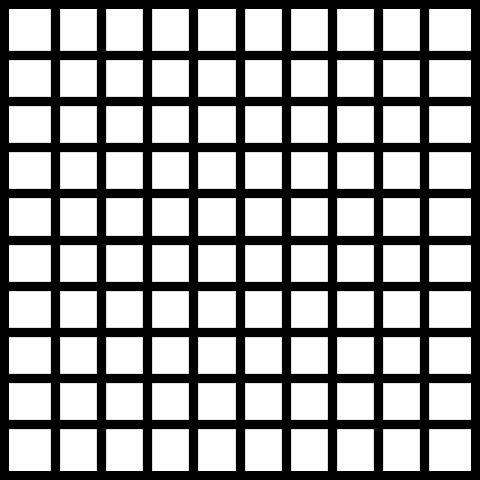
\includegraphics[scale=0.25]{rapport/2/figures/grid}
		\caption{ A 10x10 grid } \label{fig:grid}
			\end{figure}		
		
																		
		\subsubsection{Terms in the team file }
	
		\paragraph{Size}
		The size of the regiment is, in abstraction, the number of soldiers in the current regiment. 
		The size is closely connected with the total health of the regiment, as well as total damage done by the regiment.
		%The size also provides information about how much space the regiment takes up on the grid. A regiment off size $200$ would take up $200$ grid tiles.
%		One might consider it as the overall health of the regiment. While size may be an abstraction of health,
%		it's important to notice that a regiment with a larger size takes up more integers on the grid.

		\paragraph{Health}
		Health describes the initial health of each unit in the regiment.
		The total health is calculated from the size of the regiment, by using the equation\label{Total_Health} $Total\_Health = Size \times Health$.
		
		\paragraph{Attack Type}
		The Attack \textit{Type} defines how a regiment attacks. A regiments Type can only be \textit{melee} or \textit{ranged}.
		\textit{Melee} regiments can only attack regiments adjacent to their position, while ranged regiments 
		can attack any regiment within their specified range.
		
		\paragraph{Range}
		Range is an integer value, which defines how far a regiment of type \textit{ranged} can attack. 
		If a \textit{range} is defined for a regiment of type \textit{melee}, this is simply ignored.
		
		\paragraph{Damage}
		The damage of a regiment is an abstraction of the damage done by each unit in the regiment.
		The total damage done by one regiment, is calculated by the equation\label{Total_Damage} $Total\_Damage = Size \times Damage \times AttackSpeed$ 
		
		\paragraph{Movement}
		Movement defines how many tiles a regiment is allowed to move.
		
		\paragraph{Attackspeed}
		\textit{Attackspeed} governs how many attacks are performed by regiment each turn, giving units further interesting properties. 
		However, in the context of the simulation, the \textit{attackspeed} is quite simply a multiplier of the damage done by the regiment.
		
		\subsubsection{Action}
		\label{rules:action}
		When a regiment has its turn they are allowed to do the actions, \textit{attack}, \textit{MoveTowards} or \textit{MoveAway}.
		For describing these action we set a precondition(what is required to do the action), a failure(what happens if the condition is not met)
		and result(what happens if the condition is met).
		
		\paragraph{Attack action}
		\subparagraph{Usage:} 
		Attack(Regiment)
		
		\subparagraph{Precondition:} 
		\begin{itemize}\itemsep0.0001cm
		\item It is the turn of this regiment to move.
		\item For a regiment of \textit{attacktype} ranged the regiment must be in range. 
		\item For a regiment of \textit{attacktype} melee the enemy regiment must be 1 tile away(diagonals excluded).
		\item The Regiment must not have had attacked this round.
		\end{itemize}
		\subparagraph{Failure:} 
		Nothing happens
		
		\subparagraph{Result:}
		\begin{itemize} 
		\item The enemy regiment current total health pool is calculated seen \ref{Total_Health}.
		\item The total damage of the attacking regiment is calculated seen \ref{Total_Damage}.
		\item The damage is subtracted from the total health pool of the enemy regiment.
		\item The enemy regiments size is reduced by a number corresponding to the number of units that would die, in correspondence to the damage taken.
		\item The equation for calculating the new size of the attacked regiment is given by 
		\subitem \label{New_Size}$New\_Size = Size - (Damage\_taken / Health)$.
		\item If we assume, an attacking regiment that deals $2000 = 200 \times 10 \times 1$ damage, and a defending regiment that have $Health = 50$ and $Size = 200$, the resulting size of the defending regiment, after the attack, would be $200-(2000/50)=160$.
		\end{itemize}
		\paragraph{MoveTowards action}
		\subparagraph{Usage:} 
		MoveTowards(Regiment)
		
		\subparagraph{Precondition:} 
		\begin{itemize}\itemsep0.0001cm
			\item The regiment has its turn and the \textit{tiles}(Available grid-movements - left,right,up down) 
		which brings the regiment towards the target regiment is not blocked.\\
			\item The Regiment must be eligible to perform additional actions in this turn.\\
		\end{itemize}
		
		\subparagraph{Failure:} 
		Nothing happens \\
		
		\subparagraph{Result:}
		\begin{itemize}\itemsep0.0001cm
		\item The regiment will move a number of tiles equal to its movement, in the direction of the specified regiment.
		\end{itemize}
		%The regiment will move 1 tile (left,right,up down) towards the friendly/enemy regiment and movement is decreased by 1.
		
		\paragraph{MoveAway action}
		\subparagraph{Usage:} 
		MoveAway(Regiment) \\
		
		\subparagraph{Precondition:} 
		\begin{itemize}\itemsep0.0001cm
		\item The regiment has its turn and the tiles (Available grid-movements - left,right,up down)
		which brings the regiment away from the target regiment is not blocked.
		\end{itemize}
		
		\subparagraph{Failure:} 
		Nothing happens
		
		\subparagraph{Result:}
		\begin{itemize}\itemsep0.0001cm
			\item The regiment will move a number of tiles equal to its movement, in the opposite direction of the specified regiment.
		\end{itemize}
		%The regiment will move 1 tile (left,right,up down) towards the friendly/enemy regiment and movement is decreased by 1.
				
		\subsubsection{Configuration of the Playing Field}
		The simulation will need basic instructions which is a common limitation of both teams, to ensure even 'armies'. 
		As mentioned earlier this is defined in a configuration file.
		
		\paragraph{Width}
		Width defines the width of the grid measured in tiles.
		Defined with an integer value.
		
		\paragraph{Height}
		Height defines the height of the grid measures in tiles.
		Defined with an integer value.
		
		\paragraph{Standards block}
		This block will contain standard properties for regiments. These will be used if the necessary 
		information for a regiment is not entered in the main script, the regiment will use these standard properties.
		
		\paragraph{Maxima block}
		This block sets the limitations for the properties of the regiments, e.g. regiments must be of size 200 or less.

\section{Running a simulation}
%Dette skal måske ikke være her. Hvis det flyttes, så vær opmærksom på referencerne i ovenstående section, under Round og Turn
	When the simulation engine has been provided with a configuration file and two or more team files, the simulation will run. During a simulation, a lot of things happen, that are not defined in the WAR code. This section will explore these events and provide some insight in what happens during a simulation.
	
		\subsubsection{Beginning the simulation}
		When beginning the simulation, the configuration file and provided team files are read and interpreted. The information found in these files is used during the simulation. 
		
When the simulation is about to start, a team is picked at random. The chosen team is the first to evaluate its regiments turns. If there are more than two teams, the next team to go, is also chosen at random. The sequence of the teams will be consistent throughout the rounds of the simulation. All teams are added to a list of playing teams. Only teams on this list can participate in a round. When a team is initialized, each regiment related to the team, is stored in list, private to the team. This list contains all regiments, that are eligible to perform actions in a turn. 

		\subsubsection{The events of a Teams round}
		At the beginning of a teams turn, the simulation engine checks if the team is still allowed to play. 
		To be this a team must have a regiment left. Regiments are removed from a given team when their size is 0.
		If the team is allowed to play, each of the regiments on the team will have their behaviour performed.
		
%		"living" regiments. A regiment is considered living, if there is at least 1 unit left in the regiment - i.e. the regiments size must be at least 1. If the team is not eligible to play, it is removed from the list of playing teams. If there is only one team left on the list, and that team is eligible to play, that team wins the simulation. If the team is eligible to play, the simulation engine begins iterating through the regiments of the teams, performing the actions deciphered from the behaviour in the script files. Each regiments behaviour is performed in the regiments own turn - no regiment actions are performed in parallel.

		\subsection{The events of a regiments turn}
		If a given regiment is eligible to take a turn, the behaviour of the regiment is performed, 
		according to the WAR script written. If the behaviour contains one of the methods; 
		Attack, \textit{MoveTowards}, \textit{MoveAway}, they are performed, as described in section \ref{sec:describeWAR}. 
		If one or more of the three methods are performed, the grid is updated to reflect the change - 
		be it the size of an regiment or the position of a regiment. 